%\makeatletter
%\@ifundefined{standalonetrue}{\newif\ifstandalone}{}
%\@ifundefined{section}{\standalonetrue}{\standalonefalse}
%\makeatother
%\ifstandalone
%\documentclass{report}
%
%\usepackage{textcase}
\usepackage[pdftex]{graphicx}
%\usepackage{hyperref}
%\hypersetup{breaklinks=true}


% Added packages
\usepackage[usenames]{color}
\usepackage{amsfonts, amsmath, amssymb, graphics}

% NOTE: bibentry MUST appear before the hyperref or build will fail
\usepackage{bibentry}
\nobibliography*
\usepackage[square,sort,comma,numbers]{natbib}
  
\usepackage{float}
\usepackage[
    hyperindex=true,		% Make numbers of index links as well
   	backref=page, 		% Provide page listing where refs occur in the bibliography
	%breaklinks=true,
    colorlinks,%
    citecolor=green,%
    filecolor=blue,%
    linkcolor=red,%
    urlcolor=red, 
]{hyperref}

\usepackage{dsfont}
%%%% USEPACKAGES for MACROS %%%%%
\usepackage{algpseudocode}
\usepackage[chapter]{algorithm}
\usepackage{caption}
\usepackage{subcaption}
\usepackage{url}

\usepackage{array}
\usepackage{arydshln}
\usepackage{multirow}
\usepackage{multicol}
\usepackage[section]{placeins}

\newcommand{\toprule}[0]{\hline}
\newcommand{\midrule}[0]{\hline\hline}
\newcommand{\bottomrule}[0]{\hline}

\DeclareSymbolFont{AMSb}{U}{msb}{m}{n}
\DeclareMathSymbol{\N}{\mathbin}{AMSb}{"4E}
\DeclareMathSymbol{\Z}{\mathbin}{AMSb}{"5A}
\DeclareMathSymbol{\R}{\mathbin}{AMSb}{"52}
\DeclareMathSymbol{\Q}{\mathbin}{AMSb}{"51}
\DeclareMathSymbol{\PP}{\mathbin}{AMSb}{"50}
\DeclareMathSymbol{\I}{\mathbin}{AMSb}{"49}
%\DeclareMathSymbol{\C}{\mathbin}{AMSb}{"43}

%%%%%% VECTOR NORM: %%%%%%%
\newcommand{\vectornorm}[1]{\left|\left|#1\right|\right|}
\newcommand{\vnorm}[1]{\left|\left|#1\right|\right|}
\newcommand{\by}[0]{\times}
\newcommand{\vect}[1]{\mathbf{#1}}
%\newcommand{\mat}[1]{\mathbf{#1}} 

%\renewcommand{\vec}[1]{ \textbf{#1} }
%%%%%%%%%%%%%%%%%%%%%%

%%%%%%% THM, COR, DEF %%%%%%%
%\newtheorem{theorem}{Theorem}[section]
%\newtheorem{lemma}[theorem]{Lemma}
%\newtheorem{proposition}[theorem]{Proposition}
%\newtheorem{corollary}[theorem]{Corollary}
%\newenvironment{proof}[1][Proof]{\begin{trivlist}
%\item[\hskip \labelsep {\bfseries #1}]}{\end{trivlist}}
%\newenvironment{definition}[1][Definition]{\begin{trivlist}
%\item[\hskip \labelsep {\bfseries #1}]}{\end{trivlist}}
%\newenvironment{example}[1][Example]{\begin{trivlist}
%\item[\hskip \labelsep {\bfseries #1}]}{\end{trivlist}}
%\newenvironment{remark}[1][Remark]{\begin{trivlist}
%\item[\hskip \labelsep {\bfseries #1}]}{\end{trivlist}}
%\newcommand{\qed}{\nobreak \ifvmode \relax \else
%      \ifdim\lastskip<1.5em \hskip-\lastskip
%      \hskip1.5em plus0em minus0.5em \fi \nobreak
%      \vrule height0.75em width0.5em depth0.25em\fi}
%%%%%%%%%%%%%%%%%%%%%%


% \DeclareMathOperator{\Sample}{Sample}
%\let\vaccent=\v % rename builtin command \v{} to \vaccent{}
%\renewcommand{\vec}[1]{\ensuremath{\mathbf{#1}}} % for vectors
\newcommand{\gv}[1]{\ensuremath{\mbox{\boldmath$ #1 $}}} 
% for vectors of Greek letters
\newcommand{\uv}[1]{\ensuremath{\mathbf{\hat{#1}}}} % for unit vector
\newcommand{\abs}[1]{\left| #1 \right|} % for absolute value
\newcommand{\avg}[1]{\left< #1 \right>} % for average
\let\underdot=\d % rename builtin command \d{} to \underdot{}
\renewcommand{\d}[2]{\frac{d #1}{d #2}} % for derivatives
\newcommand{\dd}[2]{\frac{d^2 #1}{d #2^2}} % for double derivatives
\newcommand{\pd}[2]{\frac{\partial #1}{\partial #2}} 
% for partial derivatives
\newcommand{\pdd}[2]{\frac{\partial^2 #1}{\partial #2^2}} 
\newcommand{\pdda}[3]{\frac{\partial^2 #1}{\partial #2 \partial #3}} 
% for double partial derivatives
\newcommand{\pdc}[3]{\left( \frac{\partial #1}{\partial #2}
 \right)_{#3}} % for thermodynamic partial derivatives
\newcommand{\ket}[1]{\left| #1 \right>} % for Dirac bras
\newcommand{\bra}[1]{\left< #1 \right|} % for Dirac kets
\newcommand{\braket}[2]{\left< #1 \vphantom{#2} \right|
 \left. #2 \vphantom{#1} \right>} % for Dirac brackets
\newcommand{\matrixel}[3]{\left< #1 \vphantom{#2#3} \right|
 #2 \left| #3 \vphantom{#1#2} \right>} % for Dirac matrix elements
\newcommand{\grad}[1]{\gv{\nabla} #1} % for gradient
\let\divsymb=\div % rename builtin command \div to \divsymb
\renewcommand{\div}[1]{\gv{\nabla} \cdot #1} % for divergence
\newcommand{\curl}[1]{\gv{\nabla} \times #1} % for curl
\let\baraccent=\= % rename builtin command \= to \baraccent
\renewcommand{\=}[1]{\stackrel{#1}{=}} % for putting numbers above =
\newcommand{\diffop}[1]{\mathcal{L}#1}
\newcommand{\boundop}[1]{\mathcal{B}#1}
\newcommand{\rvec}[0]{{\bf r}}

\newcommand{\Interior}[0]{\Omega}
\newcommand{\domain}[0]{\Omega}
\newcommand{\Boundary}[0]{\partial \Omega}
%\newcommand{\Boundary}[0]{\Gamma}

\newcommand{\on}[1]{\hskip1.5em \textrm{ on } #1}

\newcommand{\gemm}{\texttt{GEMM}}
\newcommand{\trmm}{\texttt{TRMM}}
\newcommand{\gesvd}{\texttt{GESVD}}
\newcommand{\geqrf}{\texttt{GEQRF}}


\newcommand{\minitab}[2][l]{\begin{tabular}{#1}#2\end{tabular}}
\newcommand{\comm}[1]{\textcolor{red}{\textit{#1}}}

\newcommand{\nfrac}[2]{
\nicefrac{#1}{#2}
%\frac{#1}{#2}
}

\usepackage{xparse}


%%%%%%%%%%%%%%%
% Show a Author's Note
% USAGE: 
% \incomplete[Optional footnote message to further clarify note]{The text which is currently not finished}
\DeclareDocumentCommand \incomplete{ o m }
{%
\IfNoValueTF {#1}
{\textcolor{red}{Incomplete: \ul{#2}}} 
{\textcolor{red}{Incomplete: \ul{#2}}\footnote{Comment: #1}}%
}
%%%%%%%%%%%%%%%



%%%%%%%%%%%%%%%
% Show a Author's Note
% USAGE: 
% \authnote[Optional footnote message to further clarify note]{The note to your readers}
\DeclareDocumentCommand \authnote { o m }
{%
\IfNoValueTF {#1}
{\textcolor{blue}{Author's Note: \ul{#2}}} 
{\textcolor{blue}{Author's Note: \ul{#2}}\footnote{Comment: #1}}%
}
%%%%%%%%%%%%%%%



%%%%%%%%%%%%%%%
% Strike out text that doesn't belong in the paper
% USAGE: 
% \strike[Optional footnote to state why it doesn't belong]{Text to strike out}
\DeclareDocumentCommand \strike { o m }
{%
\setstcolor{red}
\IfNoValueTF {#1}
{\textcolor{Gray}{\st{#2}}} 
{\textcolor{Gray}{\st{#2}}\footnote{Comment: #1}}%
}
%%%%%%%%%%%%%%%



%
% colors to show the corrections
\newcommand{\red}[1]{\textbf{\textcolor{red}{#1}}}
\newcommand{\blue}[1]{\textbf{\textcolor{blue}{#1}}}
\newcommand{\cyan}[1]{\textbf{\textcolor{cyan}{#1}}}
\newcommand{\green}[1]{\textbf{\textcolor{green}{#1}}}
\newcommand{\magenta}[1]{\textbf{\textcolor{magenta}{#1}}}
\newcommand{\orange}[1]{\textbf{\textcolor{orange}{#1}}}
%%%%%%%%%% DK DK
% comments between authors
\newcommand{\toall}[1]{\textbf{\green{@@@ All: #1 @@@}}}
\newcommand{\toevan}[1]{\textbf{\red{*** Evan: #1 ***}}}
%\newcommand{\toevan}[1]{}  % USE FOR FINAL VERSION
\newcommand{\toe}[1]{\textbf{\red{*** Evan: #1 ***}}}
\newcommand{\tog}[1]{\textbf{\blue{*** Gordon: #1 ***}}}
%\newcommand{\togordon}[1]{\textbf{\blue{*** Gordon: #1 ***}}}
\renewcommand{\ge}[3]{{\textcolor{blue}{*** \textbf{Gordon:}\strike{#1} #2 ***}}\red{(#3)}}
\renewcommand{\ge}[3]{{\textcolor{blue}{#2}}}
\renewcommand{\ge}[3]{{\textcolor{red}{#2}}}
\newcommand{\eb}[3]{{\textcolor{red}{*** \textbf{Evan:}\strike{#1} #2 ***}}\red{(#3)}}
\renewcommand{\eb}[3]{{{\textcolor{red}{#2}}}}
%\def\ge#1#2#3{}{\textbf{\blue{*** Gordon: #2 ***}}}{(#3)}
\newcommand{\gee}[1]{{\bf{\blue{{\em #1}}}}}
\newcommand{\old}[1]{}
\newcommand{\del}[1]{***#1*** }



\input{macros/misc_mac.tex}
\newcommand{\mathsym}[1]{{}}
\newcommand{\unicode}[1]{{}}
\newcommand{\ep}{\epsilon}
\newcommand{\vx}{\mathbf{x}}


\usepackage{tabularx} 
\newcolumntype{C}{>{\centering\arraybackslash}b{1in}}
\newcolumntype{L}{>{\flushleft\arraybackslash}b{1.5in}}
\newcolumntype{R}{>{\flushright\arraybackslash}b{1.5in}}
\newcolumntype{D}{>{\flushright\arraybackslash}b{2.0in}}
\newcolumntype{E}{>{\flushright\arraybackslash}b{1.0in}}


 


\usepackage{xcolor}
% Sepia
\definecolor{myBGcolor}{HTML}{F6F0D6}
\definecolor{myTextcolor}{HTML}{4F452C}
% Dark
%\definecolor{myBGcolor}{HTML}{3E3535}
%\definecolor{myTextcolor}{HTML}{CFECEC}
%\color{myTextcolor}
\pagecolor{myBGcolor}
 
%
%\begin{document}
%\fi


\chapter{Projected Weights on the Sphere} 
\label{app:indirect_weights}

Operating on the sphere requires constrained operators described in Section~\ref{sec:projected_grad}:
\begin{align}
\mathbf{P} \cdot \nabla \phi_{k}(r(\vx)) & = \mathbf{P} \cdot \frac{(\vx-\vx_{k})}{r(\vx)} \d{\phi_{k}(r(\vx))}{r(\vx)}  \nonumber \\
& = -\mathbf{P} \cdot \vx_{k}\frac{1}{r(\vx)} \d{\phi_{k}(r(\vx))}{r(\vx)}  \nonumber \\ %\label{eq:xsfc_negative}
& = \begin{pmatrix} x \vx^{T} \vx_{k} - x_{k} \\  y \vx^{T} \vx_{k} - y_{k} \\  z \vx^{T} \vx_{k} - z_{k} \end{pmatrix} \frac{1}{r(\vx)} \d{\phi(r(\vx))}{r} \label{eq:sfc_gradient_operator}.
\end{align}
where 
\begin{align}
P = I - \mathbf{x} \mathbf{x}^T =  \begin{pmatrix} 
(1-x_1^2) & -x_1 x_2 & -x_1 x_3 \\
-x_1 x_2 & (1-x_2^2) & -x_2 x_3 \\ 
-x_1 x_3 & -x_2 x_3 & (1-x_3^2) 
\end{pmatrix} 
\label{eq:sfc_project_gradient}
\end{align}
%The operator $\mathbf{I} - \vx \vx^{T}$ for $\vx = (x,y,z)$ projects a vector onto the plane tangent to the unit sphere at $(x,y,z)$. Therefore, Equation~\ref{eq:sfc_gradient_operator} gives the projection of the gradient operator at $\vx_{k}$ onto the plane tangent to $\vx$. 

Here we investigate the difference between constructing DMs using Equation~\ref{eq:sfc_gradient_operator} on the RHS of Equation~\ref{eq:rbffd_weight_system} versus composing DMs for the standard Cartesian $\grad$ operator and combined using Equation~\ref{eq:sfc_project_gradient}.


\section{Direct Weights} 

Following \cite{FlyerLehto11}, \ref{eq:sfc_gradient_operator} takes the following form when adapted to RBF-FD:  
\begin{equation}
[ \mathbf{p}_{x} \cdot \nabla{f(\vx)}] |_{\vx = \vx_{c}} = \sum_{k=1}^{n} c_{k} \underbrace{\left[ x_{c} \vx_{c}^{T} \vx_{k} - x_{k} \right] \frac{1}{r} \d{\phi(r(x_{c}))}{r}}_{B_{c,k}^{\mathbf{p}_{x}}}. 
\label{eq:xsfc_operator_flyer_et_al}
\end{equation}
and so forth for the $\mathbf{p}_{y} \cdot \nabla, \mathbf{p}_{z}  \cdot \nabla$ operators, where $\vx_{c}$ is the stencil center and $\vx_{k}$ are stencil nodes. To compute RBF-FD weights for the $\mathbf{p}_{x} \cdot \nabla$ operator, the RHS of Equation~\ref{eq:rbffd_weight_system} is filled with elements $B_{c,k}^{\mathbf{p}_{x}}$. We will refer to this method of obtaining the weights as the \emph{direct} method due to the ability to directly compute RBF-FD weights for the operators $\mathbf{P} \cdot \nabla $, and assemble the differentiation matrices $\D_{\mathbf{p_{x}} \cdot \nabla}, \D_{\mathbf{p_{y}} \cdot \nabla}, \D_{\mathbf{p_{z}} \cdot \nabla}$ without the need to compute   and/or store other weights.

\section{Indirect Weights} 

%TODO: refer to sloan2001 for a set of test functions on the sphere that would be good test cases. 

Alternatively, weights can be computed \emph{indirectly} as a weighted combination of existing RBF-FD DMs for the unprojected $\nabla$ operator. Here we assume that differentiation matrices to compute the components of $\nabla$ are readily available in memory: 
$$
\D_{\nabla} = \begin{pmatrix} \D_{x} \\ \D_{y} \\ \D_{z} \end{pmatrix},
$$
where each matrix contains weights computed with the operators from Section~\ref{sec:rbffd_grad_weights} applied to the RHS of Equation~\ref{eq:rbffd_weight_system}.  

The differentiation matrices for $\mathbf{P} \cdot \nabla$ can then be assembled as a weighted combination of the differentiation matrices for the unprojected operator: 
\begin{equation}
\D_{\mathbf{P} \cdot \nabla} = \begin{pmatrix} \D_{\mathbf{p_{x} \cdot \nabla}} \\  \D_{\mathbf{p_{y}\cdot \nabla}} \\  \D_{\mathbf{p_{z}\cdot \nabla}} \end{pmatrix} = \begin{pmatrix} 
diag(1-X^{2}) \D_{x} - diag(XY) \D_{y} - diag(XZ) \D_{z} \\
- diag(XY)\D_{x} + diag(1-Y^{2}) \D_{y} - diag(YZ) \D_{z} \\
- diag(XZ)\D_{x} - diag(YZ) \D_{y} + diag(1-Y^{2}) \D_{z} 
\end{pmatrix}
\end{equation}
 where $X = \{x_{c,i}\}_{i=1}^{N}$, $Y = \{y_{c,i}\}_{i=1}^{N}$, $Z = \{z_{c,i}\}_{i=1}^{N}$ are the individual component values of the stencil centers $\{\vx_{c,i}\}_{i=1}^{N}$ respectively (i.e., $x_c = (x_c, y_c, z_c)$). 
%TODO: Gordon discussion: B1: explain why we use this manufactured solution. what was it designed to check.

This concept equates to classical Finite Differences where for example, the standard 5-point finite difference formula in 2-D for approximating the Laplacian can be expressed a weighted combination of coefficients for 1-D differences. 

Indirectly computing weights is of interest for at least two reasons: 
\begin{itemize}
\item The potential for memory conservation. For example, consider a coupled PDE that requires four operators: $D_x, D_y, D_z, D_{\Laplacian{}}$. A single DM on $N=10^6$ nodes with stencil size $n=101$ requires roughly $1.6$ GB of memory in double precision. Indirectly computing $D_{\Laplacian{}}$ based on the three other DMs can save a large chunk of memory. For a GPU or other accelerator (e.g., Intel Phi) with only 6 GB of global memory, the savings can be compelling.
\item The ability to compose an operator with weights loaded from disk. Possible use cases include distributing a generated grid online with precomputed RBF-FD weights for the Cartesian gradient. New investigations can reuse the grid and indirectly compose consistent operators for their problem.
%\item The cost to solve for weights and assemble DMs is $O(N*n^{3})$. The cost of adding DMs $O(N*n)$.  
\end{itemize}


\section{Comparison of Direct and Indirect Weights (INCOMPLETE)} 

%TODO: code in ~/Karen/rbffd_prototypes/matlab/stokes/test_weights

To compare direct and indirect approaches, weights are computed with each method for the MD-node sets ranging between $N = 121$ and $N=27556$. The resulting DMs for each resolution are applied to reproduce a manufactured solution. 

We monitor relative error in approximation, defined as: 
$$ \text{relative $\ell_{2}$ error} = \frac{|| f_{approx} - f_{exact} ||_{2} }{ || f_{exact} ||_{2} }, $$ 
where $f_{approx}$ is the approximate derivatives and $f_{exact}$ is the manufactured solution. 


We also look at the difference of relative errors and its absolute value: 
$$
|\text{($\ell_{2}$)}_{\text{direct}} - \text{($\ell_{2}$)}_{\text{indirect}}|
$$

We find that our indirect approach functions well compared to the direct method. For small node sizes ($N < 2500$ nodes) we see that the direct method has the advantage with 

%But the question is, how accurate is it? In situations where memory is critical and these FLOPs need to be saved (i.e., large $N$ and complicated equations), would it be useful?

%TODO: analyze results in this appendix
\begin{figure}
\begin{center}
	\centering
	\begin{subfigure}[t]{0.48\textwidth}
	\centering
	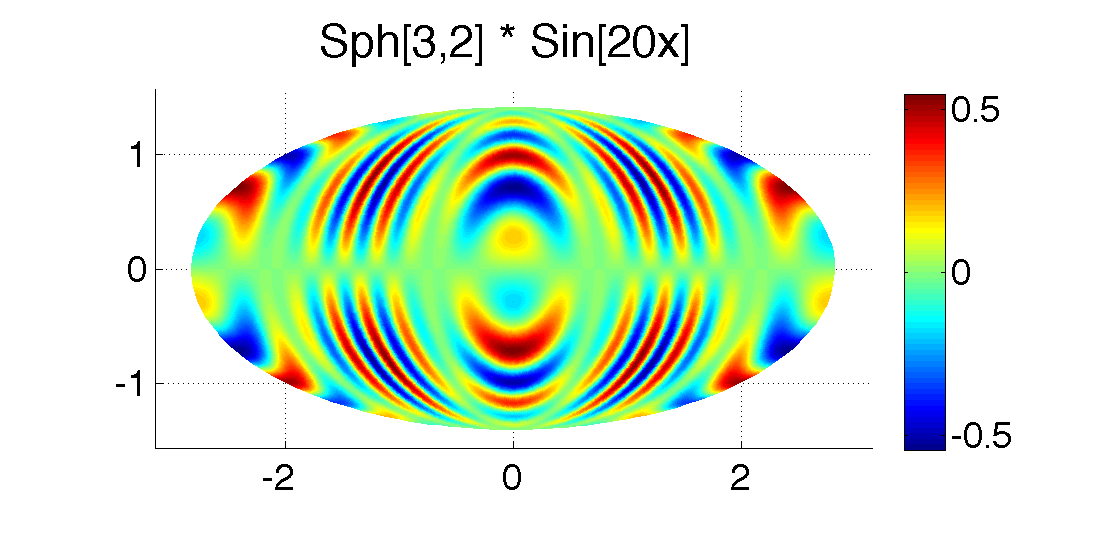
\includegraphics[width=1.0\textwidth]{../figures/appendices/direct_vs_indirect_weights/compare_weight_generation/xsfc_vs_xsfc_alt_on_sph32_times_sine_20x/sph32_times_sin20x.eps}
	\caption{Test function:  \\ $f(\vx) = Y_{3}^{2}(\vx)\sin(20x)$.  }
	\end{subfigure}
	
	\begin{subfigure}[t]{0.48\textwidth}
		\centering
	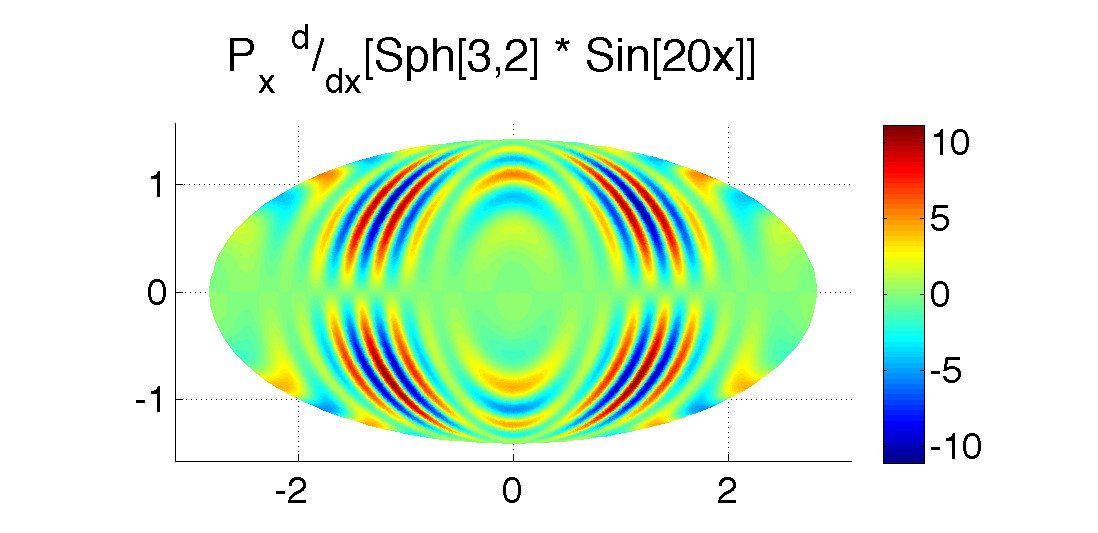
\includegraphics[width=1.0\textwidth]{../figures/appendices/direct_vs_indirect_weights/compare_weight_generation/xsfc_vs_xsfc_alt_on_sph32_times_sine_20x/pdx_sph32_times_sin20x.eps}
	\caption{Projected $x$-derivative: \\	$\mathbf{p}_{x} \cdot \nabla f(\vx)$.  }
	\end{subfigure}
	\begin{subfigure}[t]{0.48\textwidth}
		\centering
	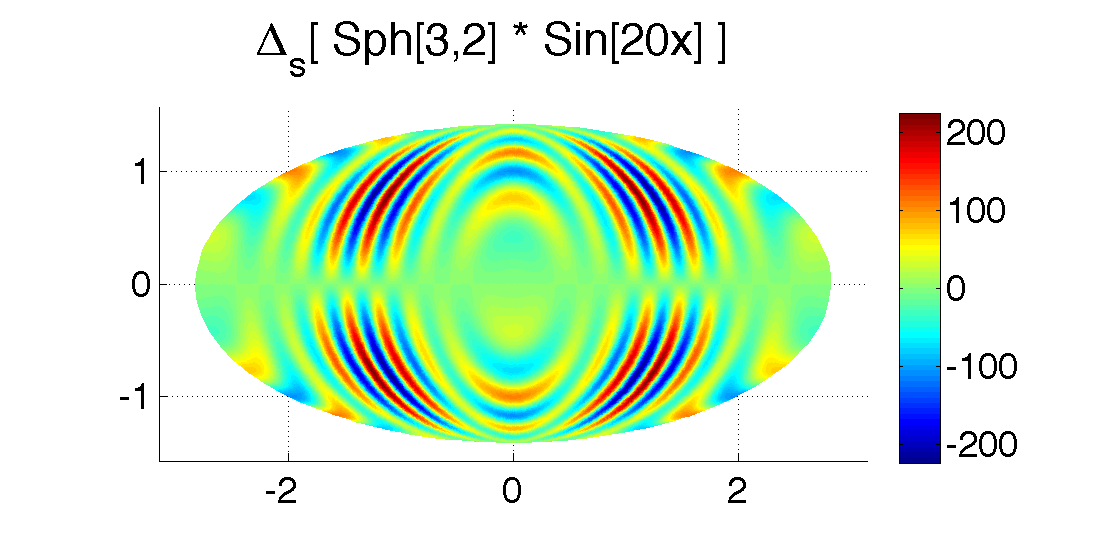
\includegraphics[width=1.0\textwidth]{../figures/appendices/direct_vs_indirect_weights/compare_weight_generation/lsfc_vs_px_grad_dot_px_grad/lsfc_sph32_times_sin20x.eps}
	\caption{Surface Laplacian: \\ $\LaplaceBeltrami f(\vx)$.  }
	\end{subfigure}
	\caption{Test function and its projected derivatives on the surface of the unit sphere. }
	\end{center}
\end{figure}

\begin{figure}
	\centering
	\begin{subfigure}[t]{0.48\textwidth}
	\includegraphics[width=1.0\textwidth]{../figures/appendices/direct_vs_indirect_weights/compare_weight_generation/xsfc_vs_xsfc_alt_on_sph32_times_sine_20x/direct_rel_l2_error.eps}
	\caption{$\mathbf{p}_{x} \cdot \nabla f(\vx)$ }
	\end{subfigure}
	\begin{subfigure}[t]{0.48\textwidth}
	\includegraphics[width=1.0\textwidth]{../figures/appendices/direct_vs_indirect_weights/compare_weight_generation/lsfc_vs_px_grad_dot_px_grad/direct_rel_l2_error.eps}
	\caption{$\LaplaceBeltrami f(\vx)$}
    \end{subfigure}
	\caption{Relative $\ell_{2}$ error in differentiation.}
\end{figure}


\begin{figure}
	\centering
	\begin{subfigure}[t]{0.48\textwidth}
	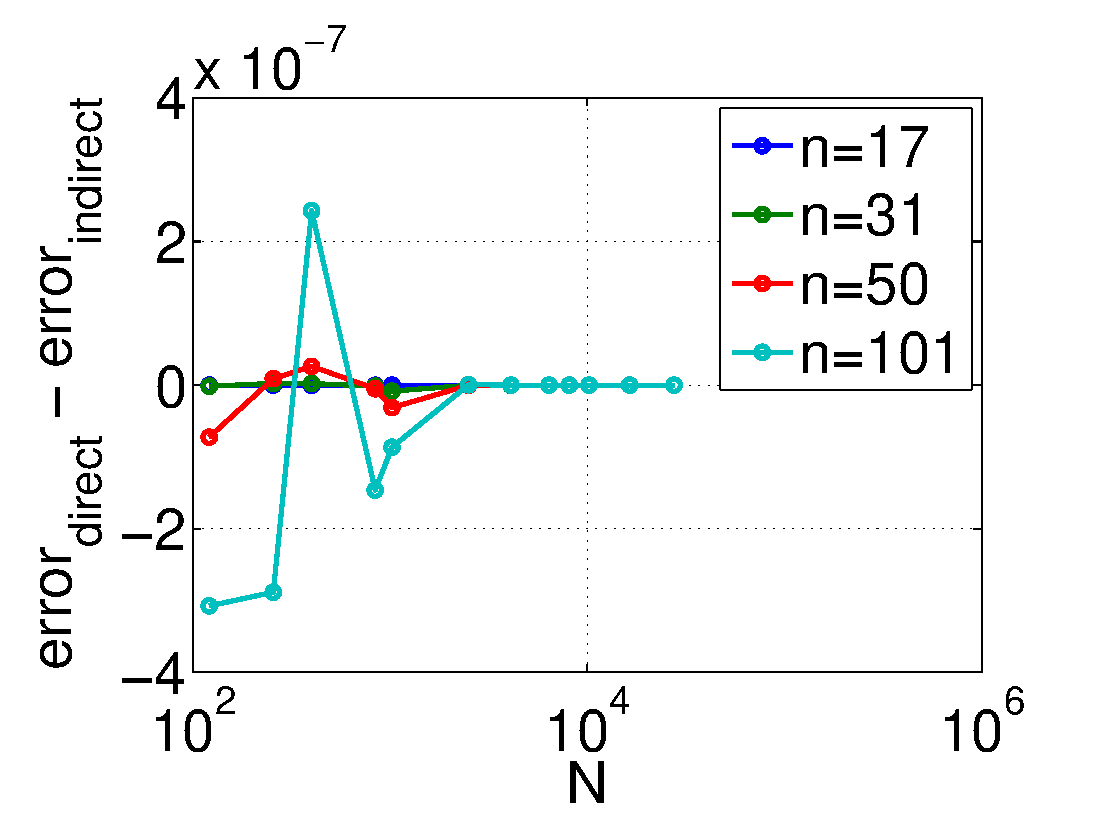
\includegraphics[width=1.0\textwidth]{../figures/appendices/direct_vs_indirect_weights/compare_weight_generation/xsfc_vs_xsfc_alt_on_sph32_times_sine_20x/diff_of_rel_l2_errors.eps}
	\caption{$\mathbf{p}_{x} \cdot \nabla ( Y_{3}^{2} \sin(20 x))$}
	\end{subfigure}
		\begin{subfigure}[t]{0.48\textwidth}
	\centering
	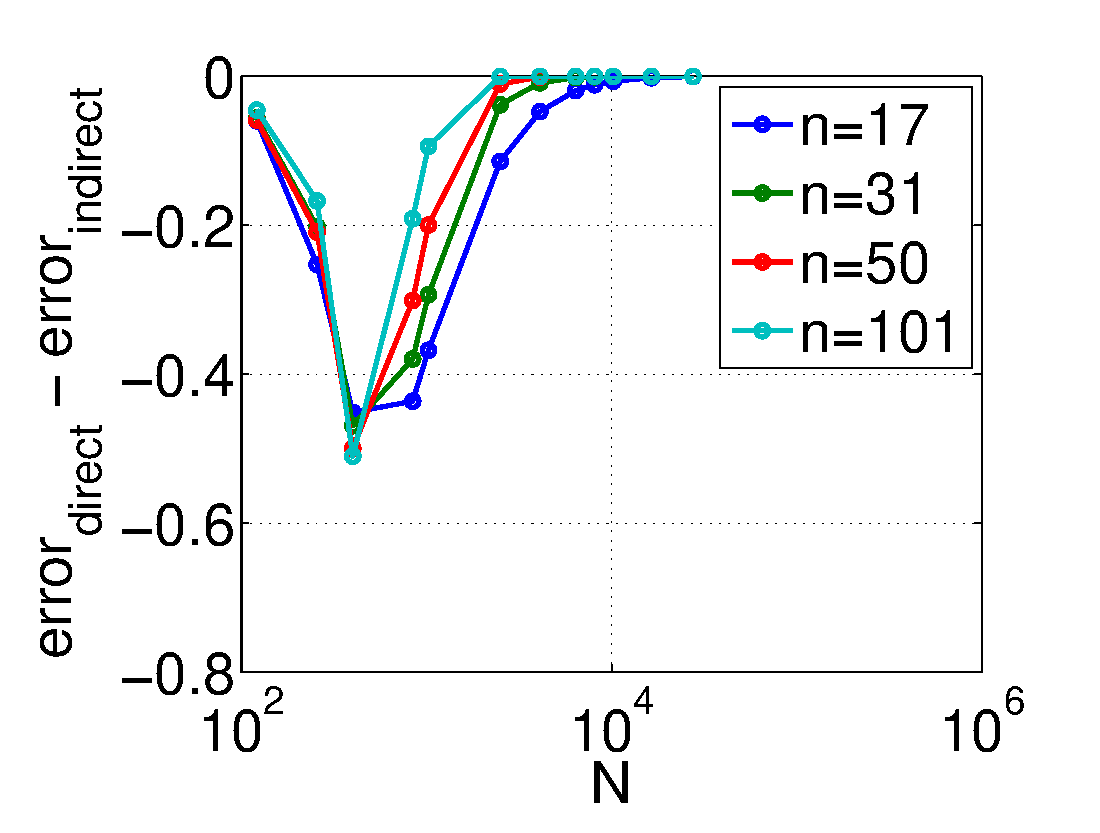
\includegraphics[width=1.0\textwidth]{../figures/appendices/direct_vs_indirect_weights/compare_weight_generation/lsfc_vs_px_grad_dot_px_grad/diff_of_rel_l2_errors.eps}
	\caption{$\LaplaceBeltrami$ of $Y_{3}^{2} \sin(20 x)$ (Indirect error is significantly higher for small resolutions. This likely due to compounding errors from the operator $P_x (D_x D_x + D_y D_y + D_z D_z)$). Where negative this figure indicates that the error is higher for indirect weight calculation. }
	\end{subfigure}
	\caption{Signed differences of relative $\ell_{2}$ errors in differentiation between Direct and Indirect weights. The sign indicates on the error indicates the higher of the two weight approaches.}
\end{figure}


\begin{figure}
	\centering
		\begin{subfigure}[t]{0.48\textwidth}
		\centering
	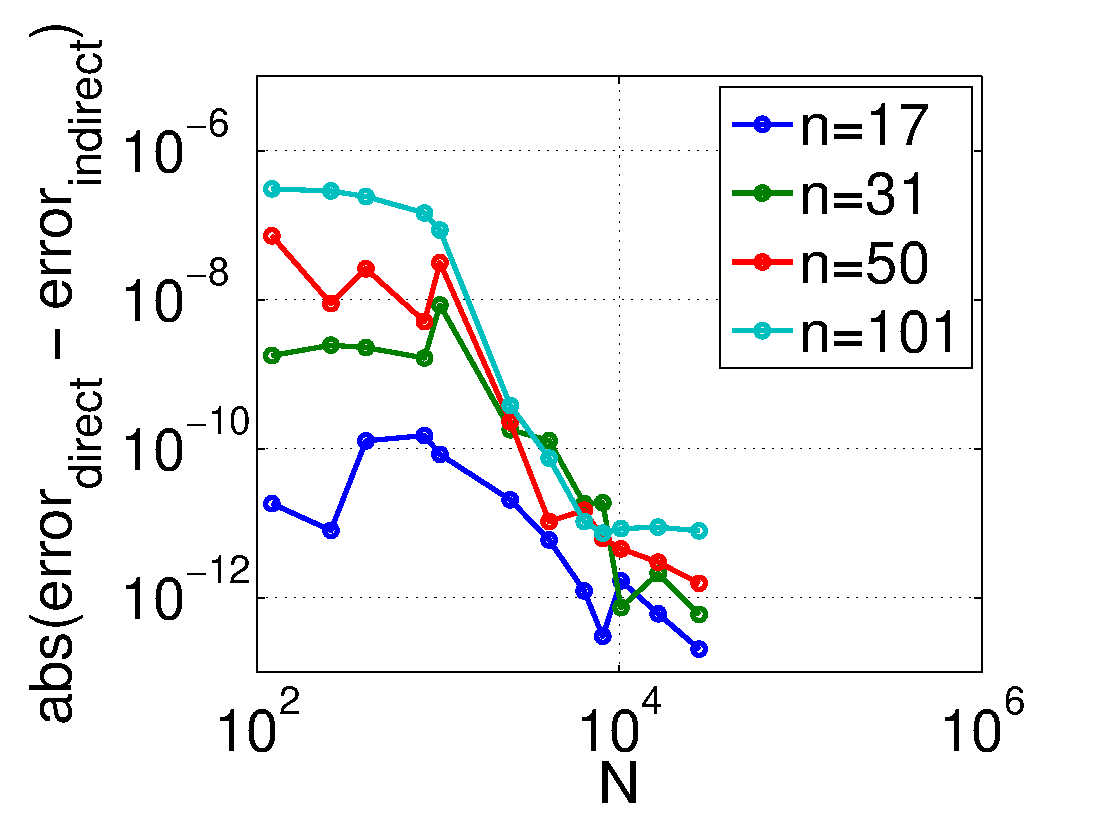
\includegraphics[width=1.0\textwidth]{../figures/appendices/direct_vs_indirect_weights/compare_weight_generation/xsfc_vs_xsfc_alt_on_sph32_times_sine_20x/abs_diff_of_rel_l2_errors.eps}
	\caption{$\mathbf{p}_{x} \cdot \nabla ( Y_{3}^{2} \sin(20 x))$}
	\end{subfigure}
	\begin{subfigure}[t]{0.48\textwidth}
	\centering
	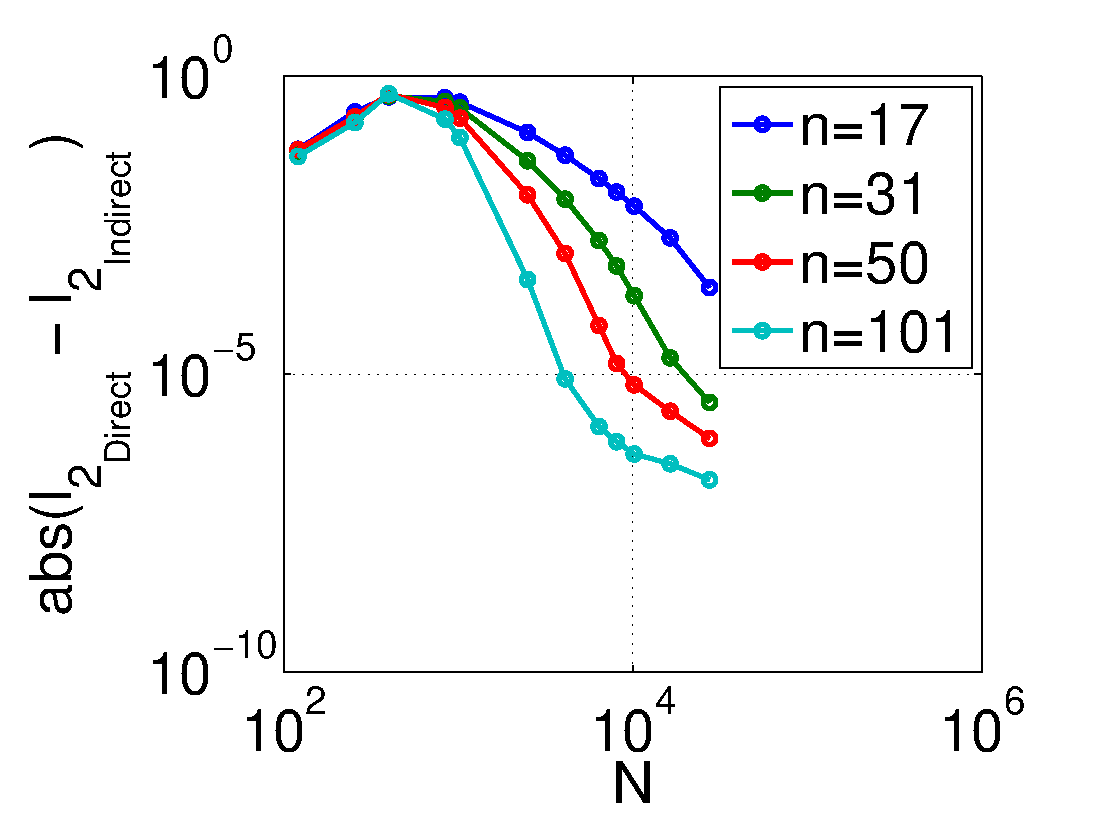
\includegraphics[width=1.0\textwidth]{../figures/appendices/direct_vs_indirect_weights/compare_weight_generation/lsfc_vs_px_grad_dot_px_grad/abs_diff_of_rel_l2_errors.eps}
	\caption{$\LaplaceBeltrami$ of $Y_{3}^{2} \sin(20 x)$}
	\end{subfigure}
		\caption{Absolute differences of relative $\ell_{2}$ errors in differentiation between Direct and Indirect weights.}
\end{figure}

%% NOT USEFUL: %%
%\begin{figure}[htbp]
%\centering
%\includegraphics[width=0.425\textwidth]{../figures/chapter2/compare_weight_generation/xsfc_vs_xsfc_alt_on_sph32/condest_dm_xsfc.pdf}
%\caption{Condition number estimates (condest) of direct $\mathbf{p}_{x}\nabla$ differentiation matrix}
%\end{figure}


\section{Conclusions}

%TODO: It appears that indirect weight calculations function. 
%TODO: They do have potential for savings
%TODO: Low resolution amplifies the errors in indirect weights. 
%TODO: still need to compare with the RBF-GA stable weight methods. What if stable weights initially resolve the extra error we see for small resolutions?




%Although it is clear the indirect method functions well compared to the direct method, we must consider its usefulness. Typically, weights are computed only as necessary for a PDE. If the PDE is on the sphere, then directly computing the $\mathbf{P}\cdot \nabla$ operator would be most efficient for both memory and computation. However, one could imagine a scenario such as a 3-D spherical shell domain with physics on the boundaries that must be constrained to the surface, while the interior requires only an unprojected $\nabla$ operator. In such cases, by simply computing for the $\nabla$ operator, we assemble all necessary operators with minimal loss of accuracy and significant savings ($3Nn$ doubles) in storage. 


%\ifstandalone
%\bibliographystyle{plain}
%\bibliography{merged_references}
%\end{document}
%\else
%\expandafter\endinput
%\fi
